% 中文阅读版。构建命令：latexmk -xelatex main_zh.tex
% 插图、参考文献和原稿的数据宏存放在同目录。
\documentclass[UTF8,fontset=fandol,scheme=chinese,zihao=false,11pt,letterpaper]{ctexart}
\usepackage[letterpaper,top=0.95in,bottom=0.85in,left=1.12in,right=1.12in]{geometry}
\usepackage{amsmath,amssymb,amsthm,mathtools}
\usepackage{graphicx,booktabs,tabularx,array}
\usepackage{algorithm,algpseudocode}
\usepackage{natbib}
\usepackage{xcolor,xurl}
\usepackage[unicode=true,colorlinks=true,linkcolor=blue!55!black,citecolor=blue!55!black,urlcolor=blue!55!black]{hyperref}
\graphicspath{{figures/}}
\hypersetup{
  pdftitle={用于数据池筛选的特征几何：效用、稳定性与局限},
  pdfauthor={匿名作者},
  pdfkeywords={数据选择, 数据池筛选, 冻结表征, 最优实验设计, 分布偏移, 实证评估},
  pdflang={zh-CN}
}
\newcommand{\R}{\mathbb{R}}
\newcommand{\E}{\mathbb{E}}
\newcommand{\tr}{\operatorname{tr}}
\newcommand{\reff}{r_{\mathrm{eff}}}
\newcommand{\cC}{\mathcal{C}}
\newcommand{\cQ}{\mathcal{Q}}
\newcommand{\norm}[1]{\left\lVert#1\right\rVert}
\newtheorem{proposition}{命题}
\newtheorem{lemma}{引理}
\renewcommand{\proofname}{证明}
\floatname{algorithm}{算法}
\algrenewcommand\algorithmicrequire{\textbf{输入：}}
\algrenewcommand\algorithmicensure{\textbf{输出：}}
\algrenewcommand\algorithmicfor{\textbf{对}}
\algrenewcommand\algorithmicforall{\textbf{对所有}}
\algrenewcommand\algorithmicwhile{\textbf{当}}
\algrenewcommand\algorithmicdo{\textbf{执行}}
\algrenewcommand\algorithmicreturn{\textbf{返回}}
\algrenewtext{EndFor}{\textbf{结束遍历}}
\algrenewtext{EndWhile}{\textbf{结束循环}}
% Generated from recorded E2b outcome tables.
\newcommand{\MainRecall}{98.333}
\newcommand{\MainRegret}{0.001311}
\newcommand{\MainReduction}{50.110}
% Supplemental diagnostics: post-hoc 2026-09-16 run.
\newcommand{\BootstrapRecall}{97.42}
\newcommand{\BootstrapMMDRecall}{97.85}
\newcommand{\BootstrapOverlap}{85.15}
\newcommand{\BrierErrorOverlap}{29.17}
\newcommand{\BrierSquaredOverlap}{30.83}
\newcommand{\BrierNLLOverlap}{90.83}
% Exploratory projection/readout follow-up, 2026-09-17.
\newcommand{\WorstErrorRecall}{40}
\newcommand{\WorstErrorGap}{1.66}
\newcommand{\ReadoutRidgeA}{98.33}
\newcommand{\ReadoutRidgeMMD}{99.38}
\newcommand{\RidgeSpan}{0.248}
\newcommand{\RidgeSelectedRegret}{0.001006}
\newcommand{\ReadoutLogisticA}{98.33}
\newcommand{\ReadoutLogisticMMD}{98.96}
\newcommand{\LogisticSpan}{14.65}
\newcommand{\LogisticSelectedRegret}{0.103}
% Exploratory decision-budget reanalysis, 2026-09-22.
\newcommand{\BudgetAFifty}{0.864511}
\newcommand{\BudgetMMDFifty}{0.864365}
\newcommand{\BudgetFull}{0.864118}
\newcommand{\BudgetRandomPrimary}{0.866030}
\newcommand{\BudgetFailureFifty}{2.083333}
% Independent matched decision timing and additive image-cost profiles.
\newcommand{\CostRidgeAResidentRatio}{0.3607}
\newcommand{\CostRidgeAImagesRatio}{1.0988}
\newcommand{\CostRidgeMMDResidentRatio}{0.1420}
\newcommand{\CostRidgeMMDImagesRatio}{1.0898}
\newcommand{\CostLogisticAResidentRatio}{0.1048}
\newcommand{\CostLogisticAImagesRatio}{0.5628}
\newcommand{\CostLogisticMMDResidentRatio}{0.1007}
\newcommand{\CostLogisticMMDImagesRatio}{0.5605}

\setlength{\parskip}{1.5pt plus 1pt}
\setlength{\emergencystretch}{1.2em}
\raggedbottom

\title{\bfseries 用于数据池筛选的特征几何：效用、稳定性与局限}
\author{匿名作者}
\date{}
\begin{document}
\maketitle
\begin{abstract}
从已有的源数据池中选择训练组合时，每试一个组合，都要拟合模型并在目标验证集上评分。按特征排序可以缩小入围名单。名单一旦确定，后续试跑就按原排名进行。当候选组合共用数据池时，前几次验证得到的损失也能用于判断哪些组合值得再试。我们从这些损失估计各池的加性贡献，据此分配剩余的拟合预算。当验证损失精确可加且能精确观测时，一组池成员指示向量满秩的查询足以确定全部候选的验证损失。我们还在共享线性模型下推导了 Target A-opt 与目标域预测风险的关系，并给出等成本的反例，其中矩匹配更好的组合反而有更高的预测风险。在 DomainNet 的逻辑回归实验中，该策略只用 25 次拟合，所选模型的平均测试 Brier 分数接近完整验证 455 次的结果。共用首批拟合时，根据验证反馈选择剩余组合，比继续按固定矩匹配排名试跑的平均测试 Brier 更低。在 Optdigits 上，重新划分同一批样本会削弱加性近似，固定筛选可能更有优势。
\end{abstract}

\section{引言}
从 15 个源数据池中选 3 个，有 455 种训练组合。各池可来自不同地点或采集条件。冻结编码器可以复用特征 \citep{radford2021,oquab2024}。每试一个组合，仍需拟合分类器，再用带标签的目标验证集评分。预算有限时，哪些组合值得试？

一种做法是先按特征给组合排序。目标感知 A-最优准则（Target A-opt）在共享线性模型下，根据目标特征上的平均预测不确定性对组合排序 \citep{yu2006,hubotter2024transductive}。使用二次核的最大均值差异（MMD）则看源域和目标域的二阶矩有多接近 \citep{gretton2012}。两种方法都用无标签的目标特征提前确定入围名单。验证分数用来决定最后保留哪个模型。即使前几次试跑的分数不理想，剩余的拟合预算也会照原排名分配。

当候选组合共用数据池时，早期的验证损失可以指导后续拟合（图~\ref{fig:pool-query-framework}）。例如，分别拟合 $A+B+C$ 和 $A+B+D$。如果各池对验证损失的影响近似可加，那么这两个分数之差也能估计在其他组合中用 $C$ 替换 $D$ 的影响。

\begin{figure}[!t]
\centering
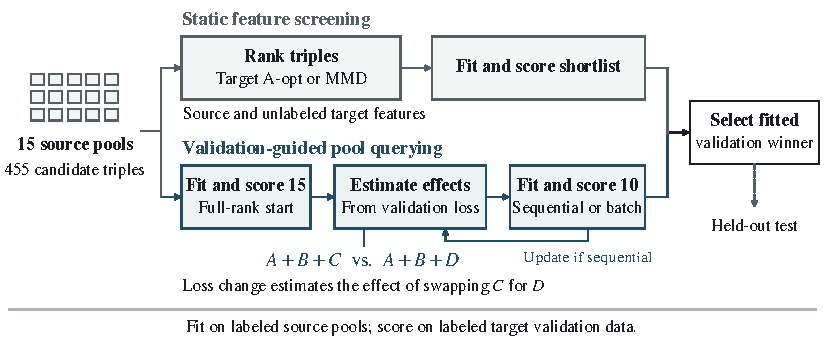
\includegraphics[width=\linewidth]{pool_query_framework.pdf}
\caption{静态筛选在拟合前确定入围名单。预算为 25 次时，池贡献查询先按成员关系选择并拟合 15 个组合，再用预测损失和杠杆值选择后 10 个。反馈箭头用于逐次查询。两条路径均从全部已拟合模型中按验证损失选出模型，再进行测试。}
\label{fig:pool-query-framework}
\end{figure}

\begin{samepage}
我们利用候选间的重叠来分配剩余拟合预算，并以固定特征排名为参照。

\begin{enumerate}
\item \textbf{用验证反馈决定后续试跑。} 先拟合一组池成员指示向量线性无关的组合，从验证损失估计各池的加性贡献。选择后续组合时，同时考虑预测损失的高低和已试跑组合的覆盖情况。后续拟合可逐次进行，也可集中在第二批，最终保留观测验证损失最低的模型。验证损失精确可加且能精确观测时，15 次线性独立查询可确定从 15 个池中选 3 个的全部组合的验证损失。

\item \textbf{解释几何筛选衡量的量。} 我们在共享贝叶斯线性模型下推导 Target A-opt 与目标域预测风险的关系，并用等样本成本的反例说明，更好的二阶矩匹配可能增加预测风险。我们也区分筛选遗漏与入围后的验证选型误差。

\item \textbf{在固定拟合预算下评估选型。} 我们在 DomainNet 和 Optdigits 上将池贡献查询与固定排名、同预算的线性实验设计及完整验证进行比较。通过共用首批拟合检验反馈的作用，通过重新划分同一批样本考察加性模型的适用性，并独立运行各策略来测量选型耗时。
\end{enumerate}
\end{samepage}

\section{相关工作}
\label{sec:related}
\subsection{目标感知实验设计}
A-最优设计以协方差矩阵的迹衡量参数不确定性 \citep{fontaine2021}。转导实验设计依据目标协变量对预测方差加权 \citep{yu2006}。ITL 和 VTL 区分可获取观测的位置与需要预测的位置，选择能降低目标熵或总方差的观测 \citep{hubotter2024transductive}。SIFT 将条件不确定性的降低用于针对提示的微调，并考虑检索样本之间的冗余 \citep{hubotter2025sift}。Target A-opt 将目标预测方差准则用于固定源池组合的排序，再用有监督评估检查入围组合。最终使用独立的有标签验证数据选出模型。

\subsection{矩匹配与数据选择}
MMD 比较分布的均值嵌入 \citep{gretton2012}。采用齐次二次核时，比较的是二阶矩。矩对齐也用于多源域适配 \citep{peng2019}。SkMM 对模型梯度构建压缩表示，以控制低秩近似偏差，再通过矩匹配控制微调中的方差 \citep{dong2024skmm}。相关的高维分析证明，在特定的合成数据增强设置中，协方差匹配是最优的 \citep{rezaei2026synthetic}。本文的 MMD 对照使用冻结特征的非中心矩，其适用性由本文的实验设置检验。

TSDS 结合基于传输的目标分布对齐，以及用于抑制近重复样本的密度感知正则项，优化采样分布 \citep{liu2024tsds}。TAROT 先对损失梯度特征进行白化，再进行基于传输的选择 \citep{feng2025tarot}。这些方法构造训练子集或采样权重。本文固定候选组合的成员关系，比较不确定性加权和直接矩匹配减少有监督评估的效果。

\subsection{特征几何与计算预算}
RankMe 通过有效秩评价表征，无需使用下游标签 \citep{garrido2023rankme}。行列式点过程倾向于选择具有互补性的子集 \citep{kulesza2012}。我们据此构建不使用目标信息的对照。计算受限的数据选择将打分与训练计入同一预算 \citep{yin2025}。选出质量更好的子集所带来的收益可能低于选择本身的成本。本文采用这一核算原则评估源池组合，同时测量最终质量及取得该质量所需的计算量。

线性最优臂识别与实验设计利用已知候选特征分配评估 \citep{soare2014linbai,fiez2019transductive,xu2018lingape,yangtan2022linbai}。本文用池成员指示向量作为候选特征，一次观测对应拟合一个读出模型，并在共享验证数据上打分。在固定协议下，观测分数是确定的，也可能偏离线性模型。采用整体反馈的组合多臂老虎机方法将观测奖励表示为各组成项奖励之和加上噪声 \citep{rejwan2020full}。我们检验线性近似对模型选型的实际作用，并纳入预留一次拟合预算以训练所推荐模型的实验设计方法。

\section{数据池选型}
\label{sec:problem}
\label{sec:theory}
\subsection{问题定义与完整流程}
数据池是一个固定的样本块。候选 $S\in\cC$ 是可行的样本块并集。入围名单的基本单位是源池组合。固定的特征映射 $h$ 包含冻结编码器和共享的无标签预处理。记 $H_i\in\R^{n_i\times d}$ 为池 $i$ 的特征矩阵，$H_S,y_S$ 分别由组合 $S$ 中的特征和标签拼接而成。所有候选共用同一个读出模型拟合规则 $\mathcal A$ 与验证损失 $L$，二者在选型前确定。

静态筛选使用源特征和无标签的目标筛选集 $T_{\rm sel}$ 确定入围名单。每个入围候选用源标签拟合，并在独立的目标验证集 $T_{\rm val}$ 上打分。算法~\ref{alg:target-a} 取 $P_0^{-1}=I$、$\sigma^2=1$，并按字典序处理并列。

\subsection{利用验证反馈查询源池组合}
\label{sec:pool-query}
一次查询用组合 $S$ 的带标签源数据拟合读出模型，并返回该模型在目标验证集上的 Brier 损失 $v(S)$。令 $x_S\in\{0,1\}^p$ 表示 $p$ 个池中哪些出现在 $S$ 中。候选组合共用数据池，因此可以用各池贡献之和近似验证损失
\begin{equation}
 v(S)=x_S^\top\beta+r(S),
 \label{eq:pool-additive}
\end{equation}
其中 $\beta$ 为池贡献系数，$r(S)$ 表示对可加性的偏离。

\noindent\textbf{选出首批 15 个组合。}
将成员指示行 $x_S^\top$ 堆叠成矩阵 $X$。在观测任何损失前，用带主元的 Gram--Schmidt 法选行，每次选离已选各行张成空间最远的一行。例如，把池按字母编号时，先选 $\mathrm{ABC}$，之后选与它没有共同池的 $\mathrm{DEF}$。全部三池组合构成的矩阵秩为 15，因此可以选出 15 个线性无关的行。这样各池贡献才有唯一估计。若秩不足，不同的贡献系数可能给出相同的已查询损失，却对未试组合给出不同预测。在损失精确可加且能精确观测的条件下，首批 15 个分数就能确定全部 455 个组合的验证损失（命题~\ref{prop:pool-identification}）。

\noindent\textbf{用新分数决定下一次试跑。}
用已查询集合 $Q$ 的成员矩阵 $X_Q$ 和观测损失 $v_Q$ 做最小二乘，得到 $\widehat\beta$。从未查询的组合中选取使下式最小的 $S$
\begin{equation}
 x_S^\top\widehat\beta-0.001\sqrt{x_S^\top(X_Q^\top X_Q)^{-1}x_S}.
 \label{eq:pool-acquisition}
\end{equation}
第一项预测损失，杠杆项使成员方向覆盖不足的组合更容易被选中。拟合所选组合后，把该组合的成员行和验证损失一并加入，再重新打分。预算为 25 次时，这个循环安排后 10 次拟合。两批法用首批 15 个验证分数只排一次序，选出剩下 10 个组合。两种做法都从全部已拟合模型中选出观测验证损失最低的一个（图~\ref{fig:pool-query-framework}，算法~\ref{alg:pool-query}）。

\subsection{目标加权不确定性为何能指导筛选}
这里的不确定性描述特征变化对预测的影响。我们采用标量贝叶斯回归形式化这一关系。设 $\theta\sim N(0,P_0)$、$P_0\succ0$，模型为 $y=h^\top\theta+\epsilon$，独立噪声满足 $\epsilon\sim N(0,\sigma^2)$ 且 $\sigma^2>0$。源与目标共享 $\theta$ 及噪声模型，目标协变量对 $\theta$ 无额外信息。记目标二阶矩为 $C_T=\E_T[hh^\top]$，则给定源设计的后验协方差与后验均值预测器的目标风险分别为
\begin{equation}
 P_S=\left(P_0^{-1}+\sigma^{-2}G_S\right)^{-1},\qquad
 R_T(S)=\sigma^2+\tr(C_TP_S).
 \label{eq:risk}
\end{equation}
该风险对后验及一个新的目标观测取平均，等于不可约噪声与目标加权参数不确定性之和。附录~\ref{app:proofs} 给出了推导。

分数 $f_A(S)=\tr(\widehat C_TP_S)$ 利用无标签目标特征估计第二项，并在固定超参数下取最小值。采用各向同性先验时，它就是转导实验设计的正则化目标方差准则 \citep{yu2006,hubotter2024transductive}。本文沿用 Target A-opt 这一名称。加入半正定的源 Gram 矩阵后，该分数至多保持原值。

对于实验所用的 $P_0^{-1}=I$ 和 $\sigma^2=1$，将 $G_S$ 写为 $G_S=U\operatorname{diag}(\lambda_j)U^\top$，包含零特征值。此时
\begin{equation}
 f_A(S)=\sum_j\frac{u_j^\top\widehat C_Tu_j}{1+\lambda_j}.
 \label{eq:target-directions}
\end{equation}
分母的倒数表示沿 $u_j$ 方向剩余的系数不确定性，分子用目标特征能量对其加权。源特征覆盖越充分，剩余不确定性越小。分子能量仅来自特征，因此没有纳入标签对该方向的重要性。即使两个组合具有相同的谱，也可能因与目标方向的对齐关系不同而获得不同分数。算法~\ref{alg:target-a} 的实现通过特征分解计算此分数，避免显式构造逆矩阵。

共享条件模型给出了 Target A-opt 的风险解释。这一假设影响风险排序。若所有特征都等于 $1$，分别由恒定标签 $+1$ 和 $-1$ 的源数据池得到两个预测器。在两个目标域中分别设置相反的恒定标签，两个预测器的风险排序就会反转，特征几何保持不变。对于分类问题，我们训练岭回归后接 softmax 的模型以及逻辑回归读出模型，测量筛选分数与这些模型的实际损失之间的关系。式~\eqref{eq:risk} 则用于共享线性回归的情形。

\subsection{矩匹配与谱对照方法}
二阶矩匹配描述源数据与目标数据的平均方向能量有多接近。令 $n_S=\sum_{i\in S}n_i$，其准则为最小化
\begin{equation}
 f_M(S)=\norm{G_S/n_S-\widehat C_T}_F^2.
 \label{eq:mmd}
\end{equation}
这是使用核 $k(h,h')=(h^\top h')^2$ 计算的经验 MMD 平方，包含对角项。它直接比较平均方向能量。两种准则使用相同的特征，因此可以检验后验不确定性所用的逆协方差加权是否比直接矩匹配带来额外收益。

有效秩在不使用目标信息的情况下概括奇异值分布的均匀程度 \citep{roy2007}。它衡量谱形状，与样本提供的证据量是不同的量，在本文用作算法~\ref{alg:target-a} 的筛选对照。附录~\ref{app:proofs} 给出有效秩的定义，以及利用组合 Gram 矩阵计算它的方法。这些对照在同一选型流程中考察源数据多样性、目标矩匹配和目标加权不确定性。

\paragraph{等成本下的风险排序反转。}
在共享线性模型中，即使精确匹配目标矩，也可能产生更高的预测风险。设每个候选包含八行单位范数的源特征，取 $G_A=\operatorname{diag}(6,2)$、$G_B=\operatorname{diag}(5,3)$，以及 $C_T=\operatorname{diag}(3/4,1/4)$。两个 Gram 矩阵的迹均为八。MMD 平方评估中，$A$ 的分数更低（$0$ 对 $1/32$）。Target A-opt 评估中，$B$ 的分数更低（$3/16$ 对 $4/21$）。附录~\ref{app:equal-cost-reversal} 给出具体构造与风险计算。

\subsection{区分筛选保留与最终选型}
筛选可能淘汰优质候选，验证选型也可能漏选入围集合中的最优候选。记 $\ell(S)$ 为固定训练预测器的目标风险，$v(S)$ 为其验证损失。若整个 $\cQ_s$ 都满足 $|v(S)-\ell(S)|\leq\varepsilon$，则验证损失极小点满足
\begin{equation}
 \ell(\widehat S)-\min_{S\in\cC}\ell(S)
 \leq
 \underbrace{\min_{S\in\cQ_s}\ell(S)-\min_{S\in\cC}\ell(S)}_{\text{筛选遗漏}}
 +2\varepsilon.
 \label{eq:decomposition}
\end{equation}
筛选遗漏比较保留集合中的最低风险和完整候选家族中的最低风险。验证选型差距为所选候选与保留集合中最优候选的风险之差。在上述偏差条件下，此差距至多为 $2\varepsilon$。该推导独立于共享线性模型假设（附录~\ref{app:proofs}）。高召回率的名单仍可能让验证程序选到质量较差的模型。即便名单缺少部分前十候选，也可能获得较低的最终损失。本文在有限测试数据上计算两种差距与召回率。

\subsection{评估预算与成本核算}
完整搜索参考方案拟合所有候选，并取 $S_{\mathrm{full}}=\arg\min_{S\in\cC}v(S)$。这一过程可实际部署。测试最优参考是观测测试损失最低的候选，仅用于审计。记 $b(S)$ 为测试 Brier 分数，即预测类别概率向量与标签独热向量之间的平均平方距离，越低越好。本文报告 $b(\widehat S_s)-b(S_{\mathrm{full}})$，以及超过预设绝对容许差的重复任务所占比例。验证排序与测试排序可能不同，因此所报告的差距可以为负。

在冻结特征可用时，筛选成本包括排序、拟合和验证入围候选。从图像开始还需计入编码器初始化与特征提取。目标感知分数也需要目标筛选集的特征。只有当包含额外特征处理在内的筛选开销小于省去的评估开销时，筛选才节约成本。候选数量与实际用时需要分别测量。计算线性筛选分数所需的矩阵运算，也可能占到岭回归拟合的相当一部分。

\section{评估协议}
\label{sec:protocol}
研究分阶段开展。合成任务用于检验风险模型。PACS 和 Office-Home \citep{li2017,venkateswara2017} 用于评估直接选型的收益是否达到预设的实际效应门槛，随后对潜在改进空间进行事后审计。之后的 DomainNet 入围名单实验在提取特征与评估结果前冻结配置。重采样、更换投影或读出模型、重新分析预算与重新分池属于探索性分析。独立计时实验另行测量执行选型流程的成本。附录~\ref{app:protocol} 记录了各项配置和结果位置。

在官方清洗版 DomainNet 数据中 \citep{peng2019}，我们按固定哈希规则选择 100 个类别。每个域的官方训练数据提供互不重叠的 1,536 张目标筛选图像、1,024 张目标验证图像和 3,072 张用于构建锚定数据池的图像，另从官方测试集中取 2,048 张图像用于测试。六个域共计 46,080 张图像。数据角色的划分将筛选、最终选型与独立评估所需的信息分开。类别元数据用于定义基准类别表，在筛选时不可用。

我们用冻结的 CLIP ViT-B/32 \citep{radford2021} 作为分池表征。各域分别按第一主成分得分划分低、中、高三个层次，每层提供一个含 512 张图像的样本块。对每个目标域，排除其自身的样本块，再枚举 $\binom{15}{3}=455$ 个组合，每个组合包含 1,536 张源图像。用于评估的特征由 ResNet-50 和 DINOv2-B/14 提供 \citep{he2016,oquab2024}。所有规则共用按行归一化、投影到 128 维的固定 Rademacher 随机投影，以及投影后的按行归一化。固定样本数量有助于将数据量与组合质量分开。共享编码器和读出模型设置使预测模型在方法对照中保持一致。

Target A-opt 取 $P_0^{-1}=I$ 和 $\sigma^2=1$。对照包括二阶矩 MMD、目标能量 $\tr(\widehat C_TG_S/n_S)$、贝叶斯 D-最优准则、合并有效秩、子空间 DPP、域平衡，以及 20 次指定种子的随机排序。各方法对同一批候选打分。域平衡还读取源域标识。核函数及并列处理规则见附录~\ref{app:protocol}。

筛选生成大小为 $10,25,50,100,227$ 的嵌套入围名单，以 $227$ 作为主要预算。在固定几何准则的对比中，U2 阶段使用岭回归独立评估每种方法的主要入围名单。岭回归的正则化系数为 $1$，无截距，softmax 温度固定。最终以验证 Brier 分数选定组合，并按字典序处理并列。同一方法的小名单复用其嵌套评估结果，各方法的缓存独立。测试阶段先验证上游哈希，再评估全部组合，以建立穷举的审计参考。

归档实验扩展到四个投影种子，并加入正则化系数固定的多项逻辑回归读出模型。该实验保留候选成员关系，并在不同入围名单的审计之间共享已拟合模型。新实验独立提取 ResNet-50 特征，对哈希分池与第一主成分（PC1）分池重新拟合，并加入人工分池的 Optdigits。在计算测试预测之前锁定每个由验证集做出的选型决策。从驻留特征起算的计时对每种策略独立重新执行。数据和拟合协议见附录~\ref{app:protocol} 和附录~\ref{app:fresh-eval}。

我们测量按测试损失排名前十的候选有多少在筛选后保留下来，并衡量验证选型与测试最优参考 $S^*$ 的差距。召回率衡量候选保留情况，遗憾度衡量相对于测试最优参考的损失差。
\begin{equation}
 \mathrm{Recall}_{10}(\cQ_s)=\frac{|\cQ_s\cap\mathrm{Top}_{10}(b)|}{10},\qquad
 \mathrm{Regret}(\widehat S)=\frac{b(\widehat S)-b(S^*)}{|b(S^*)|}.
 \label{eq:metrics}
\end{equation}
原始验收标准要求至少淘汰 $50\%$ 的候选，平均召回率至少为 $90\%$，平均归一化遗憾度不超过 $5\%$。Brier 分数为主要指标。在后续的负对数似然（NLL）和分类错误率审计中，使用对应的验证指标选型，各指标均在读取测试集之前确定。

编码器间的结果在各数据集与目标域组合内取平均，随机排序在各任务内取平均。PACS 和 Office-Home 共包含八个这样的组合，DomainNet 包含六个。后续实验的种子结果也在各域内取平均。原始自助法区间通过对目标域重采样获得。测试样本分析则固定拟合模型，并在各目标内对样本重采样。种子、编码器及相互重叠的组合均属于重复测量。

\section{实验结果}
\label{sec:results}
首先考察筛选能否在 DomainNet 上维持最终选型质量并节省计算。随后通过候选保留情况区分筛选遗漏与验证选型的影响，再通过源域对照和敏感性分析考察特征几何在何种条件下有用。共享模型实验和直接选型实验检验了几何筛选所依赖的假设。

\subsection{不同评估预算下的最终选型结果}
\label{sec:budget}
在归档投影的重新分析中，以目标域为单位计算平均值，六个域中有五个域在评估 Target A-opt 或 MMD 筛出的 50 个候选时，所得逻辑回归测试 Brier 分数低于评估 227 个随机候选的结果。两种方法与随机方法的配对平均差分别为 $-0.001518$ 和 $-0.001664$，按域进行自助法重采样所得的描述性区间分别为 $[-0.003517,0.000023]$ 和 $[-0.003720,-0.000119]$。由于共用源数据池，这些比较之间存在依赖。相对完整验证，两个预算为 50 次拟合的几何筛选方法各有 48 项重复任务中的一项，其 Brier 分数差的绝对值超过 $0.005$。将 227 次拟合的随机筛选结果按随机重复取平均，得到相应比例 $15.52\%$。上述固定预算比较使用归档拟合结果。

\subsection{基于池贡献查询的低预算选型}
\label{sec:pool-query-results}
图~\ref{fig:pool-query-results} 和表~\ref{tab:fresh-pool-query} 报告了 DomainNet 上基于冻结 ResNet-50 特征新拟合的逻辑回归结果，覆盖六个域、四个种子和两种分池方式。逐次查询 25 次在 48 个配置中的 39 个选出了与完整验证相同的模型。拟合次数仅为完整预算的 $5.5\%$，所有配置的测试 Brier 分数差均未超过 $+0.005$。按种子汇总的四个配对平均差介于 $-0.000077$ 与 $+0.000057$ 之间。与线性设计方法比较时，回放仅披露这些拟合中被查询候选的验证分数。对双编码器归档结果单独回放也发现，逐次查询 25 次的结果与固定 MMD 排序下评估 50 次的结果接近（附录~\ref{app:pool-query}）。

\begin{figure}[!t]
\centering
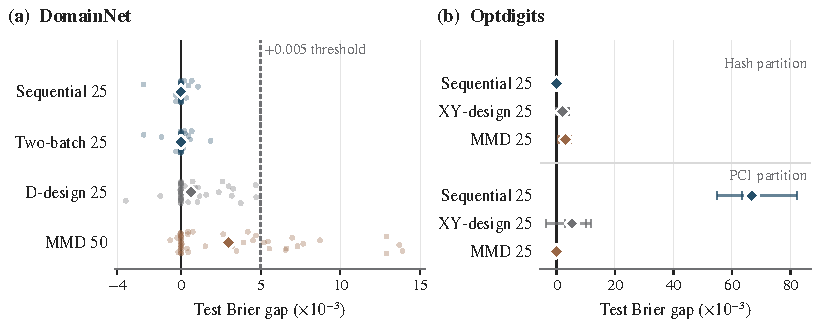
\includegraphics[width=\linewidth]{pool_query_results.pdf}
\caption{各策略选出模型的测试 Brier 分数减去通过 455 次拟合并按验证集选出的参照模型分数，零差由实线标示。菱形表示均值。(a) 点表示 DomainNet 的 48 个配置（六个目标域、四个种子、两种分池），为便于区分，点在竖直方向上略作错开。虚线标示描述性容差 $+0.005$。(b) 对每个 Optdigits 种子，两种分池使用相同的源样本。短刻线标示四个种子的结果，横线给出其取值范围。两幅子图的横轴刻度不同。D 设计和 XY 设计在 25 次拟合中各预留一次，以拟合根据预测结果推荐的候选。}
\label{fig:pool-query-results}
\end{figure}

\begin{table}[t]
\centering
\caption{DomainNet 新拟合逻辑回归模型的选型结果。均值对全部 48 个配置等权。种子间标准差按四个种子的均值计算，每个种子的均值覆盖六个域和两种分池方式。超阈值计数根据所选模型的测试 Brier 分数减去完整验证所选模型的测试 Brier 分数计算。线性设计基线在 25 次拟合中预留一次，以拟合根据预测结果推荐的候选。粗体标出 25 次拟合下最低的平均分数。}
\label{tab:fresh-pool-query}
\begin{tabular}{lrrrr}
\toprule
策略 & 拟合次数 & 测试 Brier $\downarrow$ & 种子间标准差 & 差值 $>.005$ \\
\midrule
逐次池贡献查询             & 25  & \textbf{0.916072} & 0.001431 & 0/48 \\
两批池贡献查询             & 25  & 0.916088 & 0.001412 & 0/48 \\
D 设计加推荐               & 25  & 0.916716 & 0.001537 & 0/48 \\
XY 设计加推荐              & 25  & 0.917369 & 0.001446 & 3/48 \\
LinGapE 适配版（$c=.001$） & 25  & 0.916678 & 0.001003 & 3/48 \\
Target A-opt              & 25  & 0.917241 & 0.001191 & 4/48 \\
MMD                       & 25  & 0.920236 & 0.001685 & 16/48 \\
MMD                       & 50  & 0.919060 & 0.001602 & 13/48 \\
完整验证                  & 455 & 0.916078 & 0.001451 & 0/48 \\
\bottomrule
\end{tabular}
\end{table}

固定前 15 次拟合，比较后续 10 次试跑的两种选法。与按 MMD 排名补齐相比，按拟合出的池贡献选取候选，使平均测试 Brier 分数降低了 $0.003599$。去掉杠杆项后，48 个配置中有 47 个选出了与原逐次方法相同的模型。两批版本的平均 Brier 分数与逐次版本相差不到 $0.000016$。表现最接近的线性设计基线，与逐次方法的平均测试 Brier 分数相差不到 $0.001$。附录~\ref{app:fresh-linear} 给出了全部设计基线、LinGapE 的四个系数和候选推荐规则。

图~\ref{fig:pool-query-results}(b) 考察对同一批 Optdigits 源样本重新分池的影响。采用哈希分池时，逐次查询 25 次与完整验证的分数均为 $0.299730$。按第一主成分分池后，逐次查询 25 次得到 $0.406669$，完整验证与 MMD 排序评估 25 次均得到 $0.339867$，XY 设计得到 $0.345173$。对所有候选拟合的加性模型分别解释了哈希分池和第一主成分分池中约 $85\%$ 和 $17\%$ 的验证损失变异。这项事后诊断用到了所有候选的分数。按第一主成分分池时，每个种子的 455 个候选中有 $169$--$267$ 个至少缺少一个训练类别。哈希分池下，所有候选均覆盖全部类别。类别覆盖和池间交互都可能影响上述差距。

在新 DomainNet 实验中，从特征已驻留内存开始计时。使用一个拟合工作线程时，逐次查询 25 次的耗时中位数为 $3.337$ 秒，MMD 筛选后评估 50 次为 $6.228$ 秒。使用四个拟合工作线程时，逐次查询 25 次用时 $1.922$ 秒，两批查询 25 次用时 $1.154$ 秒，MMD 筛选后评估 50 次用时 $2.069$ 秒。对于 Clipart 的一个配置，从原始图像开始计时，各策略执行一次。逐次查询 25 次、MMD 筛选后评估 50 次及完整验证分别用时 $19.60$、$23.89$ 和 $76.48$ 秒。附录~\ref{app:fresh-timing} 详细区分了这些计时设置。

\subsection{实测选型与特征成本}
\label{sec:cost}
可复用图像嵌入与少量带标签目标验证样本可用于反复选型。表~\ref{tab:cost} 报告了使用同一投影时静态筛选的配对质量和耗时。每种编码器、目标域与读出模型构成一项任务，每项任务独立完成评分、拟合和验证，重复三次。

当投影特征已驻留内存时，Target A-opt 和 MMD 各评估 50 个候选，耗时约为逻辑回归完整验证的十分之一，Brier 分数略高于完整验证，低于评估 227 个随机候选的结果。计入实测图像特征处理后，两种方法所计成本约为完整验证的 $56\%$。岭回归在不同筛选策略下的损失接近，但其单次拟合成本较低，减少拟合所节省的时间小于处理额外目标筛选特征的时间。这个成本逆转说明，即使评估次数更少，筛选开销也可能决定能否节省计算。从图像起算的成本将各项实测开销相加，池构建、下载、缓存序列化和测试审计均在计时范围之外。驻留内存特征的计时范围也不包含磁盘加载和投影。

\begin{table}[ht]
\centering
\caption{两种读出模型的最终 Brier 分数及对应的平均计入耗时，单位为秒。驻留内存的计时从投影特征已在内存中开始，包括评分、拟合和验证。图像起算的耗时在此基础上计入固定数据池清单的图像特征处理实测成本，各阶段分别计时后相加。每项均值都基于相同计时运行中的选型结果。}
\label{tab:cost}
\begin{tabular}{llrrrr}
\toprule
读出模型 & 筛选方法 & 拟合次数 & Brier & 特征驻留（秒） & 计入图像特征（秒）\\
\midrule
岭回归 & Target A-opt & 50 & 0.986655 & 0.53 & 39.59 \\
岭回归 & MMD & 50 & 0.986643 & 0.21 & 39.27 \\
岭回归 & 随机 & 227 & 0.986653 & 0.75 & 35.30 \\
岭回归 & 完整验证 & 455 & 0.986639 & 1.48 & 36.03 \\
逻辑回归 & Target A-opt & 50 & 0.863170 & 4.49 & 43.54 \\
逻辑回归 & MMD & 50 & 0.863110 & 4.31 & 43.37 \\
逻辑回归 & 随机 & 227 & 0.864241 & 21.23 & 55.77 \\
逻辑回归 & 完整验证 & 455 & 0.862992 & 42.83 & 77.38 \\
\bottomrule
\end{tabular}
\end{table}

\paragraph{岭回归校准与固定池组合的传输比较}
固定完整验证所选出的岭回归模型后，在目标验证集上拟合温度，可将测试 Brier 分数从 $0.986695$ 降至 $0.743338$，准确率均为 $36.00\%$。均匀预测的 Brier 分数为 $0.99$。划分验证集，分别用一半校准及另一半重新选型后，评估 50 次相对校准后完整验证的 Brier 分数差为：Target A-opt $-0.000150$，MMD $+0.002461$，随机筛选 $+0.016541$（附录表~\ref{tab:ridge-calibration}）。从特征已驻留内存且排名已计算的状态起算，两个 50 次筛选策略的拟合、校准和选择耗时均为 $1.114$ 秒，完整验证为 $10.047$ 秒（附录~\ref{app:server-timing}）。在新 DomainNet 的敏感性实验中，固定正则化强度并完成校准后，逐次查询 25 次在 128 维时有 0 个域相对完整验证的分数差超过 $+0.005$，在 256 维时有 3 个域超过该阈值，两种维度各评估了 6 个域。从三个正则化强度中选择时，每个候选需拟合三次（附录~\ref{app:fresh-ridge}）。

在相同的 455 个候选上使用逻辑回归读出模型，白化切片 Wasserstein 方法评估 50 个候选后得到的 Brier 分数为 $0.865342$，从驻留内存的特征计算排名耗时 $0.2948$ 秒。MMD 对应的分数和耗时为 $0.863951$ 和 $0.0387$ 秒。附录~\ref{app:calibration-transport} 给出了两种传输方法、逆协方差加权消融及实验协议的适用范围。

\subsection{候选保留与验证选型}
为区分筛选遗漏与验证选型的影响，表~\ref{tab:primary} 采用 DomainNet 原始实验结果。Target A-opt 在淘汰约一半组合的同时，几乎保留了测试 Brier 分数最低的全部十个候选。主预算下，Target A-opt 和 MMD 的每份候选短名单均包含一个在测试 Brier 上最优的候选，剩余差距来自按验证集选中了其他候选。根据公式~\eqref{eq:decomposition}，在这些短名单中，遗漏经验最优候选造成的差距为零，验证选型仍影响最终损失。

\begin{table}[t]
\centering
\caption{固定几何排序的对照在 455 个组合中保留 $s=227$ 个。均值先在各目标域内对编码器取平均，再对六个目标域取平均。召回率衡量测试 Brier 分数最低的十个候选的保留比例，遗憾值以测试 Brier 分数最低者为参照。Spearman 系数度量完整筛选排序和测试损失排序的一致性。}
\label{tab:primary}
\begin{tabular}{lrrr}
\toprule
筛选方法 & 召回率（\%） & 归一化遗憾值（\%） & Spearman 相关\\
\midrule
Target A-opt & 98.333 & 0.001311 & 0.7443 \\
二阶矩 MMD & 98.333 & 0.001311 & 0.6902 \\
贝叶斯 D-最优 & 82.500 & 0.002658 & 0.4996 \\
合并有效秩 & 81.667 & 0.002909 & 0.4951 \\
随机（20 次重复） & 48.958 & 0.003899 & 0.0016 \\
目标能量 & 46.667 & 0.009347 & -0.0399 \\
子空间 DPP & 27.500 & 0.009067 & -0.0633 \\
域平衡 & 25.000 & 0.012083 & 0.0681 \\
\bottomrule
\end{tabular}
\end{table}

主预算下，MMD 和 Target A-opt 的召回率及遗憾值相同，每个编码器与目标域组合中，两者按验证集选出的最终组合也相同。预算较低时，MMD 的平均召回率更高（附录图~\ref{fig:recall}）。完整排序的相关性衡量所有候选的整体排序一致性，召回率取决于最优候选是否进入短名单。因此，Target A-opt 较高的排序相关性未必带来更好的候选保留效果。在本实验中，两者均优于所测的不使用目标信息的规则。目标能量基线的表现更弱，说明利用目标信息的具体方式也会影响结果。

\subsection{候选构建与源域对照}
\label{sec:construction}
为检验源域构成能否提供足够的筛选信息，我们固定投影和读出模型参数，在原始分池与同一批图像的哈希分池上比较均值匹配和域级矩匹配。哈希分池由与标签和特征无关的规则确定。域级匹配先合并各源域内的所有池，再对候选所含的源域混合进行评分，因此相同源域构成的候选得分相同。附录表~\ref{app:construction-table} 给出这项探索性检验，区分随机打破并列与冻结的字典序处理规则。

重新分池后，筛选方法相对随机方法总体仍有 Brier 分数优势。预算为 50 时，域级匹配和 MMD 的平均最终 Brier 分数接近，表明这里仅利用域级矩也能获得有竞争力的全局候选短名单。均值匹配在原始分池上有竞争力，重新分池后效果下降。这些对照检验的是粗粒度信息对全局筛选是否足够。池之间能否互换需要进一步考察。

在同一源域构成内进行比较时，把从每个源域取相同池数的候选分为一组，在每个非单元素组里保留一半候选，数量向下取整。对原始分池使用逻辑回归时，Target A-opt 和 MMD 分别在约 $77\%$ 和 $76\%$ 的组中保留了经验 Brier 分数最优的候选，随机筛选为 $45\%$。重新分池后，这两个比例分别降至约 $56\%$ 和 $55\%$。用分类错误率衡量时，两者重分池后的组内保留率均低于随机。这里衡量的是各组最优候选的保留率，全局前十召回率是另一项指标。域级匹配在全局有竞争力，池级信息在组内仍可能有用，其作用随分池和评价指标而变。这两类比较仍无法量化源域构成对总体收益的因果贡献。

\subsection{投影与读出模型的敏感性}
\label{sec:readout}
在四个归档投影中，将岭回归加 softmax 换成逻辑回归后，候选间 Brier 分数的相对跨度从 $\RidgeSpan\%$ 增至 $\LogisticSpan\%$。使用这两种读出模型时，Target A-opt 平均保留测试 Brier 分数最低的十个候选中的 $\ReadoutRidgeA\%$，MMD 的保留比例略高。主预算下，两个筛选方法在每项重复任务中都保留了一个测试 Brier 分数最优的候选。若按分类错误率计算，Target A-opt 的召回率最低为 $\WorstErrorRecall\%$（附录~\ref{app:diagnostics}）。

\subsection{共享风险模型下的目标加权}
在 216 个合成设置中，与表现最好的无目标信息有效秩基线相比，Target A-opt 将模型所定义的线性风险降低 $4.23\%$。与 MMD 相比，下降 $14.85\%$。先在每个设置内对种子求平均，再对设置重采样，得到的描述性 95\% 区间分别为 $[3.86,4.62]\%$ 和 $[13.99,15.70]\%$。在单独的条件分布偏移实验中，平均归一化实际预测遗憾值由无偏移时的 $0.211$ 增至最大测试偏移下的 $3.143$。

\subsection{直接选型与可用改进空间}
PACS 和 Office-Home 用于检验筛选分数能否直接选出更好的源池组合。在池数预算为 $K=3$ 时，按配置计算 Brier 分数的相对改善再取平均，Target A-opt 相比 DPP 和 MMD 的改善幅度分别为 $0.351\%$ 和 $0.273\%$。两者均低于预设的 $2\%$ 实际效果阈值。与 DPP 的配对差区间跨过零，与 MMD 的配对差区间为负。具体数值见附录~\ref{app:diagnostics}。这些对照固定的是池数，源样本数可随组合而变。
事后的全量审计用测试损失最小的候选与参照作比较，度量能够取得的改进空间。相对 DPP 的平均改进空间仅为 $0.781\%$，反映了平均收益的局限，预设检验仍未达到效果阈值。因此，有必要分别衡量预测改进和评估工作量减少。PACS 和 Office-Home 为理解结果提供背景。等样本成本筛选需要另外检验。

\section{讨论}
\label{sec:discussion}
\subsection{筛选在什么条件下有用}
评价筛选应考察完整的选型过程。最终损失用于判断减少评估次数后能否取得可接受的选择，筛选遗漏和验证选型的诊断则有助于解释质量损失。实际计时用来确认是否节省计算。不同读出模型下观察到的成本逆转对此尤为关键。单次拟合的成本本来就低时，有用的候选短名单也可能带来额外开销。
MMD 和域级匹配的表现说明，评价细粒度几何方法时应包括简单的匹配基线。全局筛选可以在域级信息下取得有竞争力的结果。在源域混合构成固定时，池级信息仍可能有用。选择运行配置时，应综合目标指标、可接受的损失差距与实测成本。召回率和完整排序相关性分别只刻画其中一部分。

\subsection{局限性}
\label{sec:limitations}
DomainNet 的多个目标域共享源数据，不同种子是在同一基准上的重复测量。Optdigits 使用人工构建的数据池。固定预算查询验证的是 15 个池组成 455 个候选的设置，如何可靠地选取预算及从少量观测分数中检测加性失效仍是开放问题。减少查询次数时仍复用同一组目标验证标签。超过 $0.005$ 的计数和种子间波动描述的是所测配置。

由几何推导的风险适用于共享线性回归模型。标签生成机制的变化、读出模型的选择和概率评价指标的变化均可能改变分类实验结果。静态方法以图像为起点的成本是独立实测的各环节开销之和，从原图运行池贡献查询的直接计时覆盖一个 Clipart 配置。池准备成本及编码器预训练数据重叠问题未纳入检验。

\section{结论}
\label{sec:conclusion}
当加性池贡献能够预测验证损失随组合的变化时，可利用候选间的池重叠及验证反馈，在较低预算下选择源池组合。新 DomainNet 实验中，拟合 25 次所得的测试 Brier 分数接近完整验证，分批查询在并行拟合时可缩短耗时。Optdigits 实验表明，改变分池方式后，几何筛选可能更有优势。特征成本、读出模型和损失结构共同决定何种选型配置有效。

\label{main-text-end}

\subsection*{人工智能使用说明}
生成式人工智能工具用于协助重述概念、起草数学命题和证明、设计实验、实现软件、解读结果、检索文献、撰写论文、编写绘图脚本和翻译中文。本文报告的数值来自实际记录的实验材料。人工智能的辅助不构成对这些材料或数学结论的独立验证。提交版本应由作者核查，作者对其负责。

\subsection*{可复现性说明}
附录~\ref{app:proofs}、\ref{app:pool-query} 和 \ref{app:fresh-eval} 提供证明、查询协议、新实验的数据与计时流程，以及线性实验设计的比较规则。第~\ref{sec:protocol} 节和附录~\ref{app:protocol} 说明预处理、数据访问规则、候选构造、指标及结果路径。\href{https://github.com/anonymization26/collapsemodel/blob/a4f317a0b50fed229019e4559e88530d3ebc11c8/Rebuttal/README.md}{复现仓库}提供原始与修订实验的代码、已记录的结果和核验命令。实验清单中的哈希值可用于核对大型特征缓存。

\subsection*{伦理说明}
本研究使用已有基准图像和预训练编码器，无须招募新的参与者。数据公开可用并不消除图像许可、隐私或表征偏差方面的顾虑。特征谱多样性和较高的入围召回率，都不足以表明所选数据池具有社会代表性、公平性或隐私保护。候选池的分类方式、与预训练数据是否重叠的不确定性，以及任务仅限视觉分类，均限制了本文对下游部署的主张。数据和模型的访问仍受原始使用条款约束。

\bibliography{references}
\bibliographystyle{iclr2027-style/iclr2027_conference}
\clearpage
\appendix

\section{数学结论的证明与适用范围}
\label{app:proofs}
奇异值分解 $H=U\Sigma V^\top$ 将特征方向与各方向的强度分开。固定非负权重 $w_i$ 后，将缩放后的源特征矩阵按行拼接，得到
\begin{equation}
 G_S=H_S^\top H_S=\sum_{i\in S}w_iG_i.
 \label{eq:gram}
\end{equation}
该和矩阵的特征值等于合并后特征矩阵的奇异值平方。预处理坐标系固定时，它保留各方向的强度及不同源数据池在这些方向上的对齐关系。实验采用单位权重。

有效秩将奇异值归一化为概率向量，再对其熵取指数 \citep{roy2007}：
\begin{equation}
 \reff(H)=\exp\!\left(-\sum_j p_j\log p_j\right),\qquad
 p_j=\frac{\sigma_j(H)}{\sum_k\sigma_k(H)}.
 \label{eq:rank}
\end{equation}
对非零矩阵，约定 $0\log0=0$，且 $1\leq\reff(H)\leq\operatorname{rank}(H)$。所有正奇异值相等时取上界。两个奇异值之比为 $9:1$ 时，有效秩约为 $1.38$。两个奇异值相等时，有效秩为二。用 Gram 矩阵计算时，要先对特征值开平方再归一化。直接归一化特征值会得到另一个指标。重复整个矩阵不改变有效秩，因此它刻画谱的形状。在本文实验中，有效秩作为无需目标域信息的对照指标。

给定 $H_S$ 及高斯似然，对先验与似然乘积中的指数项配方，得到后验精度矩阵 $P_0^{-1}+\sigma^{-2}H_S^\top H_S$ 和后验均值 $\mu_S=P_S\sigma^{-2}H_S^\top y_S$。对独立的目标域观测 $y=h^\top\theta+\epsilon$，给定训练数据和 $h$ 有
\begin{equation}
 \E[(y-h^\top\mu_S)^2\mid H_S,y_S,h]=\sigma^2+h^\top P_Sh.
\end{equation}
对 $h$ 积分即得式~\eqref{eq:risk}。这里假设目标域协变量的分布不提供该模型以外关于 $\theta$ 的额外信息。若某个源域采用不同的回归函数，或任务为多类别分类且使用 softmax 读出模型，推导得到的风险与实际评估损失一般不同。该证明未给出模型设定偏差的上界。以有限样本估计代替 $C_T$ 还会引入估计误差。

设 $S_Q$ 是 $\cQ_s$ 中使 $\ell$ 最小的候选。由候选清单上的一致偏差界可得
\begin{equation}
 \ell(\widehat S)\leq v(\widehat S)+\varepsilon
 \leq v(S_Q)+\varepsilon\leq\ell(S_Q)+2\varepsilon.
\end{equation}
两边减去 $\min_{S\in\cC}\ell(S)$ 即得式~\eqref{eq:decomposition}。该代数推导给出的是条件式。若要据此得出总体上的泛化结论，还需结合实际依赖结构和选型规则，证明一致偏差事件以何种概率成立。仅在有限测试集上穷举候选无法完成这一步。

在 Frobenius 内积下，特征映射 $\phi(h)=hh^\top$ 满足 $\langle\phi(h),\phi(h')\rangle_F=(h^\top h')^2$。因此，源域和目标域经验特征均值的平方距离即式~\eqref{eq:mmd}。这是保留对角项的有偏经验平方 MMD，对应 V 统计量。该量由未中心化二阶矩决定，具有相同二阶矩的分布会得到相同的结果。本文将其作为计算简便、使用相同信息的筛选对照。

\subsection{等成本下矩匹配与目标风险的排序反转}
\label{app:equal-cost-reversal}
取单位基向量 $e_1,e_2$，目标分布在这两个向量上分别赋予概率 $3/4$ 和 $1/4$。设一个共同的四行源池块包含这两个基向量各 $(3,1)$ 次，另有两个备选的四行源池块，出现次数分别为 $(3,1)$ 和 $(2,2)$。将共同块与任一备选块合并，得到 $G_A=\operatorname{diag}(6,2)$ 或 $G_B=\operatorname{diag}(5,3)$，两者均有八个样本且迹为八。由于 $G_A/8=C_T$，而 $G_B/8-C_T=\operatorname{diag}(-1/8,1/8)$，相应平方 MMD 分别为 $0$ 和 $1/32$。在共享的高斯线性模型中，取单位先验精度和单位观测噪声方差，两个后验协方差矩阵分别为 $\operatorname{diag}(1/7,1/3)$ 和 $\operatorname{diag}(1/6,1/4)$。用 $C_T$ 加权后的风险项分别为 $4/21$ 和 $3/16$。两者共有的不可约噪声项相消，故 $A$ 的预测风险比 $B$ 高 $1/336$。

\section{实现与审计细节}
\label{app:protocol}
最初的 DomainNet 实验拟合岭回归读出模型，并将其分数转换为类别概率。权重和 Brier 损失为
\begin{equation}
 \begin{aligned}
 W_S&=(I+G_S)^{-1}\sum_{i\in S}H_i^\top Y_i,\qquad
 p(x)=\operatorname{softmax}(h(x)^\top W_S),\\
 b(S)&=\frac1{n_T}\sum_t\norm{p(x_t)-e_{y_t}}_2^2.
 \end{aligned}
\end{equation}
$Y_i$ 为固定 100 类标签空间中的源标签独热矩阵。该实验不拟合截距，也不调节温度。以 float32 载入特征后，以 float64 执行线性代数运算。由 Gram 矩阵的特征分解计算有效秩时，将舍入产生的负特征值截断为零，开平方得到奇异值，仅保留满足 $\sigma_j>\sigma_{\max}\sqrt{8\epsilon_{64}\max(n_S,d,1)}$ 的项。代码对零矩阵返回秩零。该容差用于判定数值秩，熵的定义保持原样。共享投影使用种子 $20260911$ 和维度 $d=128$。锁定的 DomainNet 方案事先确定维度。

贝叶斯 D-最优 最大化 $\log\det(I+G_S)$。子空间 DPP 取每个池块 Gram 矩阵的前 16 个特征向量 $U_i$，定义 $K_{ij}=\norm{U_i^\top U_j}_F^2/16$ 且 $K_{ii}=1$，再通过数值投影得到半正定相关矩阵，并最大化 $\log\det(K_{S,S}+10^{-8}I)$。这里的核刻画池块的子空间。域平衡分数为组合覆盖的域数，减去各域池块数平方之和的 $10^{-3}$ 倍，取此分数最大者。确定性评分遇到并列时，按组合标识符的字典序处理。这些方案是预先固定的对照。该 DPP 构造的表现仅适用于此项实现。

DomainNet 记录图像内容哈希、样本标识、官方划分的归属、用途分配和类别词表。提取特征前核验归档及划分文件的校验和。各用途的样本互不重叠，并检查内容是否完全重复，以处理已构建基准内部的重叠。语义近重复和预训练数据污染仍有可能。各筛选方法使用相同的源池块、投影、目标筛选样本和候选集。特征提取忽略标签。构建基准时利用分类体系的元数据，并存储标签供后续获准使用的阶段读取。

筛选、验证和审计清单将配置和上游产物的哈希绑定在一起。各阶段的加载器分别控制对标签和数据划分的访问。原始方案中，验证分别评价每种方法或每次随机重复。锁定选择后，测试审计覆盖每个编码器的全部 $6\times455$ 个组合。在测试集上穷举得到的最优候选仅供研究参考。下文说明后续研究的缓存方案。

种子 $20260917$、$20260918$、$20260919$ 和 $20260920$ 生成新的 128 维 Rademacher 投影，投影前后均进行相同的逐行归一化。种子 $20260911$ 用于核验实现，另四个种子的均值不含此对照。逻辑回归采用 L2 正则化，$C=1$，无截距，使用 LBFGS，容差为 $10^{-6}$，最多迭代 1,000 次。出现收敛警告时中止该任务。实验中未出现收敛警告，实际最多迭代 24 次。类别词表固定，对源样本中缺失的类别赋予零概率。

各方法沿用各自的筛选规则，并保留候选组合和五种候选清单大小。筛选、拟合与验证，以及冻结模型后的测试，由独立流程执行。审计在读取测试特征前核验源数据、配置、产物来源、模型和选型结果的哈希。后续实验为每种读出模型拟合每个组合一次，供多种方法复用。缓存的穷举评估支持对不同候选清单进行反事实比较。Brier、NLL 和错误率均按各自对应的验证损失完成选型。原始种子下的岭回归复现了 5,460 个重建的测试组合，最大损失差为 $1.78\times10^{-15}$，并精确复现全部 1,620 个基于 Brier 的验证选择。

两个编码器、五个种子和两类读出模型共进行 54,600 次拟合。对新种子的汇总先在任务内对随机重复取均值，再在每个目标域内对编码器和种子取均值，最后对六个域取均值。每类读出模型有 48 次编码器、种子和域的组合测量。它们仍对应六个共享相同源数据池的域级单位。

匿名代码归档记录图像与特征哈希，并提供结果表。DomainNet 配置位于 \path{code/configs/target_conditioned_e2b/domainnet_v1.json}，实验位于 \path{results/target_conditioned/e2b_fixed_cost_shortlist/domainnet_v1/}。投影与读出模型的归档位于 \path{results/target_conditioned/revision_20260917/}。固定成本下的预算、构造和计时记录位于 \path{results/target_conditioned/revision_20260922/}。

\begin{algorithm}[htbp]
\caption{Target A-opt 筛选与验证}
\label{alg:target-a}
\begin{algorithmic}[1]
\Require 源数据池 $\{D_i\}$、候选集 $\cC$ 及目标域集合 $T_{\rm sel},T_{\rm val}$。
\Require 固定特征映射 $h$、拟合规则 $\mathcal A$、损失 $L$ 及候选清单大小 $1\leq s\leq|\cC|$。
\Ensure 候选清单 $\cQ_s$、选中的组合 $\widehat S$ 和拟合后的读出模型 $q_{\widehat S}$。
\State 用 $h$ 构造 $H_i$ 和 $H_{\rm sel}$，此步骤不读取标签。
\State 缓存 $G_i=H_i^\top H_i$，估计 $\widehat C_T=H_{\rm sel}^\top H_{\rm sel}/|T_{\rm sel}|$。
\For{每个 $S\in\cC$}
  \State $G_S\gets\sum_{i\in S}G_i$，$f_A(S)\gets\tr\!\left[\widehat C_T(I+G_S)^{-1}\right]$。
\EndFor
\State 按 $(f_A(S),\operatorname{id}(S))$ 排序，保留前 $s$ 个候选作为 $\cQ_s$。
\For{每个 $S\in\cQ_s$}
  \State 利用源标签拟合 $q_S\gets\mathcal A(H_S,y_S)$。
  \State $v(S)\gets |T_{\rm val}|^{-1}\sum_{(x,y)\in T_{\rm val}}L(q_S(h(x)),y)$。
\EndFor
\State 在 $\cQ_s$ 中选择使 $(v(S),\operatorname{id}(S))$ 最小的 $\widehat S$。
\State \Return $\cQ_s,\widehat S,q_{\widehat S}$。
\end{algorithmic}
\end{algorithm}

\subsection{静态筛选核验}
\label{app:diagnostics}
表~\ref{app:construction-table} 在投影和样本成本固定时比较哈希重分池与原始分池。对每个域，用确定性哈希将相同的 1,536 张图像分为三个池块，目标数据的用途分配保持不变。域匹配使用源域的矩进行比较，因此域组成相同的候选会并列。事后随机化对照使用 20 个预先锁定的并列排序并取均值。在每个含多个候选的域组成层内保留一半候选时，如果对并列候选进行均匀随机排序，仅依赖域组成的匹配方法保留最优组合的期望恰为 $45.68\%$。图~\ref{fig:recall} 给出各预算下的召回率。

PACS/Office-Home 上，$K=3$ 时，Target A-opt、DPP 和 MMD 的平均 Brier 分数分别为 $0.826769$、$0.829162$ 和 $0.828719$。Target A-opt 减去两种基线的配对差异区间分别为 $[-0.007449,0.000731]$ 和 $[-0.003392,-0.000712]$。事后审计遍历每个任务的 220 个组合。历史 DomainNet 投影实验中，Target A-opt 对测试错误率最低的候选召回率最小的情形为 DINOv2/Quickdraw、逻辑回归及种子 $20260918$。该候选清单仍包含测试错误率最小的候选。

第~\ref{sec:cost} 节的静态计时从已驻留内存的投影特征开始。对每个编码器、目标域和读出模型，各方法独立完成排名、拟合和验证，重复三次。直接以图像为起点时，还计入初始化、输入输出、特征提取和投影。构造候选与测试审计的时间单独处理。

\begin{figure}[t]
\centering
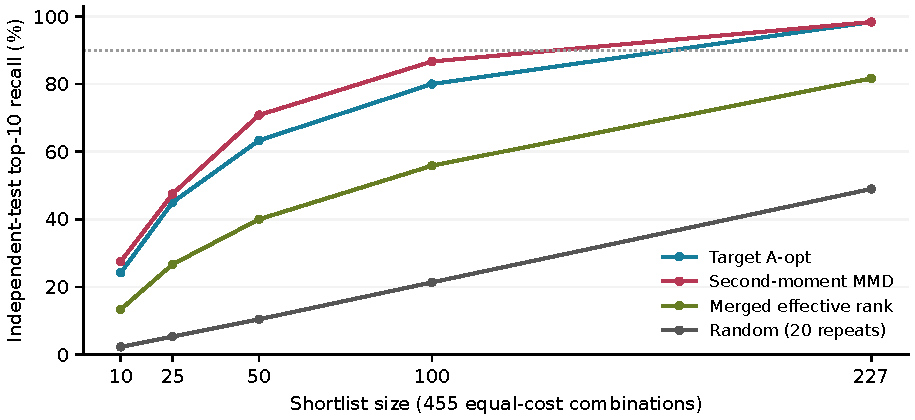
\includegraphics[width=\linewidth]{shortlist_recall.pdf}
\caption{原始 DomainNet 实验中，不同候选清单大小下测试 Brier 分数最优的十个候选的平均召回率。点线为预先规定的召回率阈值。各曲线使用同一组候选组合，并按相应规则使用特征。}
\label{fig:recall}
\end{figure}

\begin{table}[ht]
\centering
\caption{分池构造对照使用逻辑回归的 Brier 分数。$s=50$ 时，报告验证选中的组合的最终损失。最后几列统计在每个至少包含两个候选的域组成层内保留一半候选时，是否保留经验最优候选。先对目标域内的分层和编码器取均值，再对六个目标域取均值。域匹配的最终损失为 20 种随机并列排序下的均值。层内结果采用均匀处理并列时的精确期望。}
\label{app:construction-table}
\begin{tabular}{lrrrr}
\toprule
 & \multicolumn{2}{c}{最终 Brier 分数 ($s=50$)} & \multicolumn{2}{c}{同域组成内的保留率 (\%)}\\
筛选方法 & 原始分池 & 哈希分池 & 原始分池 & 哈希分池\\
\midrule
Target A-opt & 0.863170 & 0.869699 & 77.22 & 55.83 \\
MMD & 0.863110 & 0.869257 & 76.11 & 55.00 \\
均值匹配 & 0.863713 & 0.873038 & 75.28 & 57.78 \\
域二阶矩匹配（平局随机） & 0.863667 & 0.869356 & 45.68 & 45.68 \\
随机 & 0.870013 & 0.874244 & 45.04 & 45.31 \\
\bottomrule
\end{tabular}
\end{table}

\section{逐次池贡献查询}
\label{app:pool-query}

\begin{proposition}[精确可加条件下的可识别性]
\label{prop:pool-identification}
考虑从 15 个源数据池中选取三个池得到的全部组合。若每个候选 $S$ 均满足 $v(S)=x_S^\top\beta$，且每次查询精确返回 $v(S)$，则任何一组由 15 个查询行组成的满秩设计所对应的 15 个分数，均能确定全部候选的验证分数。
\end{proposition}
\begin{proof}
每个池出现在 $\binom{14}{2}=91$ 个三池组合中，每对池共同出现在 $\binom{13}{1}=13$ 个组合中。因此，完整的成员指示矩阵满足 $X^\top X=78I+13\mathbf{1}\mathbf{1}^\top\succ0$。满秩查询设计 $X_Q$ 给出的唯一系数向量为 $X_Q^{-1}v_Q$。将其左乘 $X$ 得到完整损失向量。由于任一候选均满足 $x_S^\top\mathbf{1}=3$，截距可由已有系数表示。当查询少于 15 次时，沿 $X_Q$ 零空间中的任意非零方向扰动系数，所有已查询值保持不变，且至少改变一个未查询值。因此，对一般情形，即使允许自适应查询，少于 15 次查询仍不足以确定完整损失表。围绕各分量均为一的常量损失向量施加充分小的扰动，可使两张损失表均落在 Brier 分数的取值范围内。
\end{proof}

该命题针对给定拟合与验证方案下实际测得的验证损失面。真实损失可以偏离可加性，系数是用于近似的模型参数。若要得到未查询的预测最优组合对应的拟合读出模型，仍需额外查询一次。算法~\ref{alg:pool-query} 可将下一次查询分配给探索，并返回已观察到的最优候选。杠杆值项为启发式设计，未作置信度校准。

\begin{algorithm}[H]
\caption{利用验证反馈查询源池组合}
\label{alg:pool-query}
\begin{algorithmic}[1]
\Require 秩为 $p$ 的候选成员矩阵 $X$、预算 $p\leq B\leq|\cC|$、查询模式及拟合和验证接口。
\State 用贪心主元 Gram--Schmidt 法从 $X$ 中选取 $p$ 行。
\State 拟合并验证这些候选，以初始化 $Q$ 和 $v_Q$。
\While{$|Q|<B$}
  \State 拟合 $\widehat\beta\gets\arg\min_\beta\|v_Q-X_Q\beta\|_2^2$。
  \State 按式~\eqref{eq:pool-acquisition} 的分数由低到高对未查询候选排序。
  \State 取排名第一的候选（逐次法）或排名前 $B-|Q|$ 的候选（两批法）。
  \State 拟合并验证所选候选，将成员行和观测损失并入 $Q$ 和 $v_Q$。
\EndWhile
\State \Return 使 $(v(S),\operatorname{id}(S))$ 最小的已查询候选及其拟合读出模型。
\end{algorithmic}
\end{algorithm}

初始化时，每轮将未选行投影到已选各行张成的空间，选取平方残差最大的一行。平方残差和查询分数均舍入至小数点后 12 位，并列时按候选标识符字典序处理。将 15 个池标为 $A$ 至 $O$ 时，各行初始平方范数均为 $3$，所以先选 $\mathrm{ABC}$。接下来，$ABD$ 的平方残差为 $3-2^2/3=5/3$，而 $\mathrm{DEF}$ 的平方残差仍为 $3$。完整顺序为
\[
\begin{gathered}
 \mathrm{ABC,\ DEF,\ GHI,\ JKL,\ MNO,\ ADG,\ AEH,\ AFI,}\\
 \mathrm{BJM,\ BKN,\ BLO,\ DEI,\ DHJ,\ DKM,\ JKO}.
\end{gathered}
\]
前五个组合已覆盖全部池，但只给出了五个独立的和。之后的十个主元各增加一个独立方向。满列秩使 $X_Q^\top X_Q$ 可逆，加入新的查询行之后仍保持满秩。15、25 和 50 的查询预算使用相互嵌套的查询序列前缀。几何偏移消融采用相同的初始化和查询规则，以 $v(S)-g(S)$ 为响应变量做最小二乘拟合，再将 $g(S)$ 加回预测分数。当候选数为 $N=455$ 且排名从零开始时，$g(S)=0.005[\operatorname{rank}_A(S)+\operatorname{rank}_M(S)]/[2(N-1)]$。仅利用池贡献的规则始终设 $g(S)=0$。

归档回放先锁定查询轨迹，再进行测试审计。四组额外投影复用六个目标域和两个编码器下已拟合模型的损失。逐次查询 25 次、固定 MMD 50 次和完整验证的平均测试 Brier 分数分别为 $0.864174$、$0.864365$ 和 $0.864118$。按投影种子和目标域形成的 24 个配对均值，对两个参照的差均不超过 $+0.005$。预算为 25 次时，加入几何偏移后，48 个配置中有两个选中了不同候选，平均 Brier 分数上升 $0.000007$。

\section{固定候选成员下的校准与传输对照}
\label{app:calibration-transport}
两项核验均采用原始 DomainNet 的源池成员、六个目标域、两个编码器和投影种子 20260911。先在每个域与编码器的组合内对随机排序取均值，再在域内对编码器取均值，最后对六个域等权汇总。各质量差均以相对应的 455 次完整验证所选模型的测试 Brier 分数为参照。

\subsection{岭回归温度校准}
\label{app:ridge-temperature}
岭回归正则化参数保持 $\lambda=1$。重建所有候选的 $T=1$ 分数后，12 个配置中，验证 Brier 分数的最大偏差为 $1.95\times10^{-9}$，测试 Brier 分数的最大偏差为 $1.86\times10^{-9}$。测试对照仅用于核验重建。给定候选的类别分数 $z$，在从 $0.01$ 到 $100$ 的 81 个对数等距温度值上评估 $\operatorname{softmax}(z/T)$，取使验证 Brier 分数最小的 $T$。

首先，对各配置固定原始完整验证选中的模型，用全部 1,024 个验证样本拟合温度。平均测试 Brier 分数由 $0.986695$ 降至 $0.743338$，Top-1 准确率仍为 $36.00\%$。均匀概率预测的参照为 $1-1/100=0.99$。随后，按固定样本 ID 哈希划分验证集。每个候选的温度在其中 512 个样本上拟合，在另 512 个样本上选型。最终测试前锁定温度和所选候选。表~\ref{tab:ridge-calibration} 报告重新选型的结果。预算为 227 次拟合时，两种几何筛选在全部 12 个配置中均找到了校准后完整验证选中的候选。校准实验的特征维度和岭回归正则化固定。附录~\ref{app:server-timing} 给出采用独立验证子集时的计算成本。

\begin{table}[ht]
\centering
\caption{在互不重叠的两个验证子集上分别拟合温度和重新选型后，岭回归的表现。最后一列统计相对校准后完整验证的域级平均测试 Brier 差严格超过 $+0.005$ 的域数。}
\label{tab:ridge-calibration}
\begin{tabular}{rlrrrr}
\toprule
拟合次数 & 筛选方法 & 测试 Brier & Top-1 准确率 & Brier 差 & 域数 \\
\midrule
50 & Target A-opt & 0.725347 & 37.63\% & $-0.000150$ & 1/6 \\
50 & MMD          & 0.727958 & 37.61\% & $+0.002461$ & 2/6 \\
50 & 随机       & 0.742038 & 36.35\% & $+0.016541$ & 5/6 \\
227 & Target A-opt & 0.725498 & 37.78\% & $+0.000000$ & 0/6 \\
227 & MMD          & 0.725498 & 37.78\% & $+0.000000$ & 0/6 \\
227 & 随机       & 0.730224 & 37.37\% & $+0.004726$ & 2/6 \\
455 & 完整验证 & 0.725498 & 37.78\% & $+0.000000$ & 0/6 \\
\bottomrule
\end{tabular}
\end{table}

\subsection{同候选的切片 Wasserstein 对照}
\label{app:transport-fixed}
我们在同一组 455 个固定池组合上评分，并使用几何筛选所用的相同冻结源特征和无标签目标筛选特征。对 32 个固定的高斯随机单位方向，分别对候选的 1,536 个样本与目标域的 1,536 个样本的投影值排序，再计算两个有序序列的对应值之差的平方均值。最后对这 32 个距离取均值。白化变体使用合并后的中心化源特征协方差矩阵的逆平方根，岭正则化系数取其平均特征值的 $0.1$ 倍。每个编码器与目标域的组合共用一种变换，所有候选使用同一个变换。该对照检验固定候选条件下基于最优传输的对齐。TAROT \citep{feng2025tarot} 使用有监督的损失梯度特征，在样本级进行选择。

重新计算的Target A-opt 和 MMD 排名与配对读出归档中所有前 50 和前 227 个候选的集合一致。我们先锁定排名，再用归档的逻辑回归验证损失选型，并用测试损失审计。表~\ref{tab:fixed-transport} 报告排名耗时。每个配置从已驻留内存的投影特征开始，单线程运行三次并取中位数，必要时计入白化。再对各配置取平均。第~\ref{sec:cost} 节另报告静态筛选的计时研究，包含拟合和验证并核算特征提取成本。227 次拟合时，四种几何筛选相对完整验证的平均差的绝对值均小于 $0.0005$。

\begin{table}[ht]
\centering
\caption{固定候选池上的传输对照，使用逻辑回归读出与 50 次拟合预算。Brier 差以 455 个候选的完整验证为参照。耗时为从内存中已驻留的投影特征开始计算排名所用的秒数。}
\label{tab:fixed-transport}
\begin{tabular}{lrrrr}
\toprule
筛选方法 & 测试 Brier & Brier 差 & 秒 & 域数 $>+0.005$ \\
\midrule
切片 Wasserstein & 0.866406 & $+0.002649$ & 0.2777 & 1/6 \\
白化切片 Wasserstein & 0.865342 & $+0.001585$ & 0.2948 & 0/6 \\
Target A-opt & 0.864104 & $+0.000347$ & 0.5482 & 0/6 \\
MMD & 0.863951 & $+0.000194$ & 0.0387 & 0/6 \\
随机 & 0.871557 & $+0.007800$ & \textemdash & 4/6 \\
完整验证 & 0.863757 & $+0.000000$ & \textemdash & 0/6 \\
\bottomrule
\end{tabular}
\end{table}

\subsection{逆协方差加权与校准岭回归耗时}
\label{app:server-timing}
在同一组 DomainNet 逻辑回归候选上使用 50 次拟合预算时，Target A-opt 的平均测试 Brier 分数为 $0.864104$，省略逆协方差加权的线性目标能量为 $0.896467$，MMD 为 $0.863951$。

我们单独对采用两个独立验证子集、$\lambda=1$ 的岭回归方案计时，从已驻留内存的投影特征和预先计算的排名开始，计入池块统计量的计算、拟合、温度搜索和最终选型。Target A-opt 50 与 MMD 50 均耗时 $1.114$ 秒，完整验证为 $10.047$ 秒。汇总时对 12 个编码器与域的组合分别取三次运行中位数，再取均值。温度搜索约占校准方案耗时的 $93$--$94\%$。

\section{新增评估与线性实验设计对照}
\label{app:fresh-eval}

\subsection{基准与锁定的选型方案}
\label{app:fresh-protocol}
我们重新获取数据并开展了新的有监督拟合实验。清洗后的 DomainNet 划分包含 345 类，并在拟合前依据固定哈希选择其中 100 类。六个域各从官方训练划分中提供 1,536 张源图像、512 张无标签目标筛选图像和 1,024 张目标验证图像，三类用途之间互不重叠。每个域从官方测试划分中留出 2,048 张测试图像。对任一目标域，其余五个域各提供三个含 512 张图像的源池。每个候选在三个池的 1,536 张图像上训练。特征由在 ImageNet 上预训练的冻结 ResNet-50 提取，随后随机投影至 128 维，投影前后均做行归一化。四个种子改变投影与哈希分池。第二种分池方式在每个源域内，沿中心化源特征的第一主成分（PC1）对图像排序，再划分成等大的池。两种构造使用相同的图像集合。

对 Optdigits \citep{alpaydin1998optdigits}，每个种子从官方训练划分取 3,000 个样本，按哈希或源特征的 PC1 人为构造 15 个池，每池 200 个样本。官方测试划分来自不同的书写者。我们按样本 ID 的哈希，将其分为 256 个无标签筛选样本、512 个验证样本和 1,029 个留出的测试样本。读出模型的输入为原生 64 维计数特征，按 $1/16$ 缩放后逐行归一化。沿用相同的四个种子，评估种子与分池方式组成的全部八个配置。

两个基准均使用多项逻辑回归，$C=1$，无截距，L-BFGS 容差为 $10^{-6}$，最多迭代 1,000 次。预测与固定标签词表对齐，训练中缺失的类赋予零概率。所有候选选择均在测试评估前锁定。每种策略只能查看已查询候选的验证损失，455 次拟合的参照也按验证损失选定。对同一入选模型，报告测试 Brier 分数、Top-1 准确率和负对数似然（NLL）。计算 NLL 时将概率下限设为 $10^{-15}$。在 DomainNet/PC1 上，与 MMD 25 相比，逐次查询 25 次的平均测试 Brier 更低（$0.909862$ 对 $0.913940$），但 NLL 更高（$4.011643$ 对 $3.858980$）。不同种子使用相同的底层基准数据。$+0.005$ 是描述各配置相对完整验证的差距的阈值。随机策略在每个配置内对 20 种锁定排序取均值。

\subsubsection{可加近似的诊断}
对 Optdigits，使用全部 455 个验证分数拟合可加模型，哈希分池的 $R^2$ 为 $0.851$，PC1 分池为 $0.169$。查询 25 次后，在仍未查询候选上的预测 $R^2$，哈希分池为 $0.637$，PC1 分池为 $-7.57$。这些诊断使用选型时不可见的分数。若在部署时检查可加假设，需要额外查询未用于拟合的候选，并将这些查询计入预算，因为 15 个线性独立的查询行足以插值拟合最初的 15 个分数。

\subsection{线性最优臂识别与实验设计}
\label{app:fresh-linear}
本文的每个臂对应一个池组合，其已知特征为 15 维池成员指示向量，奖励取为验证损失的相反数。线性最优臂识别和转导实验设计已利用共享特征信息推断最优候选 \citep{soare2014linbai,fiez2019transductive}。在本文固定的验证任务中，重复评价一个候选会得到相同的分数。池间交互可能使损失系统性地偏离线性模型。这里的 $0.001$ 探索系数是启发式参数。

后续实验在同样的 48 个 DomainNet 配置和八个 Optdigits 配置上，对新拟合得到的验证分数做仅揭示所查分数的回放。基准此前已用于分析，但新增基线的结果产生之前已固定比较协议。所有基于成员指示向量的方法均以同样的 15 个线性独立行初始化，并对已查询的分数作普通最小二乘拟合。预算按不同候选的拟合次数计算，以 25 为主要预算，另用 50 和 100 作核验。令 $V$ 为已查询指示行的 Gram 矩阵。对可能的下一行 $x$，贪心 D-design 最大化 $x^\top V^{-1}x$。A-design 最小化更新后 Gram 矩阵的逆的迹。G-design 最小化候选行的最大预测方差，XY-design 最小化候选两两分数之差的最大预测方差。这些是指示向量模型下的单步实验设计。Target A-opt 则使用定义在分类器特征上的目标加权准则。本文的有限预算 LinGapE 变体 \citep{xu2018lingape} 根据预测差距及其不确定性确定当前预测最优者和一个挑战者，再查询能使二者差距的不确定性最小的未用行。该变体使用相同的 15 行初始化，固定的四个缩放系数为 $0.001$、$0.01$、$0.1$ 和 $1$。

所有改造后的基线均可先按各自策略查询 $B-1$ 次，再拟合一个尚未查询且预测最好的候选，最后返回 $B$ 次拟合中验证损失最低的模型。我们还检查两种做法：将全部 $B$ 次拟合分配给策略并返回观测最优模型，或在获得第 $B-1$ 次拟合后预测的候选模型时直接返回该模型。所有选择均在测试审计前锁定。在 DomainNet/PC1 上，预留这一次拟合将 D-design 相对完整验证的平均测试 Brier 差由约 $0.0128$ 降至 $0.0010$。在 Optdigits/PC1 上，XY-design 将平均验证遗憾值，即相对最低验证损失的差，由逐次查询 25 次的 $0.059715$ 降至 $0.009403$。表~\ref{tab:fresh-linear-breakdown} 按分池方式报告预算匹配的对照。在本任务中，原始 OD-LinBAI 需要更高的名义预算 \citep{yangtan2022linbai}。使用 41--43 次不同候选的拟合时，其相对表现取决于分池和终止规则。

\begin{table}[!htb]
\centering
\caption{线性实验设计对照中，按数据集和分池构造汇总的测试 Brier 分数。低预算方法均拟合 25 个候选。D/A/G/XY 设计和 LinGapE 变体预留一次拟合，以实现其推荐的预测最优候选。池贡献查询的消融方法、MMD 和Target A-opt 均在各自查询过的候选中选取验证分数最优者。}
\label{tab:fresh-linear-breakdown}
\begin{tabular}{lrrrr}
\toprule
 & \multicolumn{2}{c}{DomainNet} & \multicolumn{2}{c}{Optdigits} \\
\cmidrule(lr){2-3}\cmidrule(lr){4-5}
策略 & 哈希 & PC1 & 哈希 & PC1 \\
\midrule
逐次查询 & 0.922283 & 0.909862 & 0.299730 & 0.406669 \\
两批查询 & 0.922263 & 0.909912 & 0.300364 & 0.406669 \\
仅利用 & 0.922283 & 0.909940 & 0.299730 & 0.406669 \\
D-design & 0.922524 & 0.910907 & 0.300751 & 0.406229 \\
A-design & 0.922502 & 0.911131 & 0.302644 & 0.376545 \\
G-design & 0.922509 & 0.911892 & 0.300364 & 0.371922 \\
XY-design & 0.922463 & 0.912276 & 0.301795 & 0.345173 \\
LinGapE 变体，$c=0.001$ & 0.922291 & 0.911066 & 0.302299 & 0.403567 \\
LinGapE 变体，$c=0.01$ & 0.922551 & 0.910722 & 0.301396 & 0.403567 \\
LinGapE 变体，$c=0.1$ & 0.922711 & 0.910773 & 0.301733 & 0.406669 \\
LinGapE 变体，$c=1$ & 0.922634 & 0.910854 & 0.301726 & 0.380168 \\
MMD & 0.926531 & 0.913940 & 0.302909 & 0.339867 \\
Target A-opt & 0.922727 & 0.911755 & 0.304332 & 0.339867 \\
完整验证（455 次拟合）& 0.922216 & 0.909941 & 0.299730 & 0.339867 \\
\bottomrule
\end{tabular}
\end{table}

\subsection{逻辑回归的独立计时}
\label{app:fresh-timing}
特征驻留内存后的计时独立运行排名或查询计算、拟合与验证。DomainNet 使用六个目标域、哈希分池和第一个种子。Optdigits 使用哈希分池下的第一个种子。每种策略在每个配置下轮换顺序重复三次，每个拟合工作线程使用一个 BLAS 线程。缓存解码、完整性检查和测试评分单独处理。

\begin{table}[!htb]
\centering
\caption{单个或四个拟合工作线程下，从特征驻留内存开始的逻辑回归选型耗时（秒）。DomainNet 项为 18 次运行的中位数，Optdigits 项为三次运行的中位数。}
\label{tab:fresh-logistic-time}
\begin{tabular}{lrrrr}
\toprule
 & \multicolumn{2}{c}{DomainNet} & \multicolumn{2}{c}{Optdigits} \\
\cmidrule(lr){2-3}\cmidrule(lr){4-5}
策略 & 单线程 & 四线程 & 单线程 & 四线程 \\
\midrule
逐次查询 25 & 3.337 & 1.922 & 0.552 & 0.642 \\
两批查询 25 & 3.284 & 1.154 & 0.526 & 0.762 \\
MMD 25 & 3.168 & 1.107 & 0.550 & 0.897 \\
MMD 50 & 6.228 & 2.069 & 1.092 & 1.630 \\
Target A-opt 25 & 3.223 & 1.347 & 0.614 & 0.867 \\
完整验证 & 59.585 & 19.243 & 9.632 & 12.223 \\
\bottomrule
\end{tabular}
\end{table}

对于预先选定的 Clipart/哈希配置，我们还在 V100 上从本地图像与预训练权重开始，对完整流程计时。每种策略都从尚未提取特征的状态出发，使用一个拟合工作线程运行一次，计入模型加载、图像输入输出和变换、特征提取、投影与选型。逐次查询、两批查询和完整验证各编码 8,704 张图像。MMD 还需编码 512 张无标签目标筛选图像。四种策略的总耗时分别为 $19.602$ 秒（逐次 25）、$19.646$ 秒（两批 25）、$23.885$ 秒（MMD 50）和 $76.480$ 秒（完整验证）。统计范围未包含下载、Python 导入及强制清空操作系统缓存的时间。这是一项 Clipart 案例研究，每种方法运行一次。

\subsection{岭回归校准与特征维度敏感性}
\label{app:fresh-ridge}

使用 DomainNet 哈希分池的首个种子，考察五种嵌套投影。在验证集的前一半上，从 $0.01$ 到 $100$ 的 81 个对数等距值中选择温度。联合调参的实验组还从 $\lambda\in\{0.1,1,10\}$ 中选择正则化系数，因此每个候选需要三次有监督拟合。所有实验组均使用验证集的后一半完成选型，共用几何排名。表~\ref{tab:fresh-ridge-sensitivity} 在相同校准设置下比较各方法。

\begin{table}[htbp]
\centering
\caption{新增 DomainNet 岭回归敏感性分析，采用哈希分池和首个种子。Brier 分数在六个域等权平均。计数列统计逐次查询 25 次相对采用该列校准与正则设置的完整验证，测试 Brier 差严格超过 $+0.005$ 的域数。}
\label{tab:fresh-ridge-sensitivity}
\begin{tabular}{r rrr rrr}
\toprule
 & \multicolumn{3}{c}{校准，固定 $\lambda$} & \multicolumn{3}{c}{校准，调优 $\lambda$} \\
\cmidrule(lr){2-4}\cmidrule(lr){5-7}
维度 & 逐次 25 & 完整验证 & 域数 & 逐次 25 & 完整验证 & 域数 \\
\midrule
64  & 0.880595 & 0.878260 & 2/6 & 0.880624 & 0.877666 & 2/6 \\
96  & 0.846247 & 0.844187 & 2/6 & 0.844467 & 0.843555 & 1/6 \\
128 & 0.827308 & 0.827477 & 0/6 & 0.830918 & 0.827681 & 1/6 \\
256 & 0.785407 & 0.780673 & 3/6 & 0.779687 & 0.776171 & 2/6 \\
512 & 0.752150 & 0.753835 & 1/6 & 0.745405 & 0.749862 & 1/6 \\
\bottomrule
\end{tabular}
\end{table}

\subsection{规模和预算的探索性核验}
在构造的 Clipart 排名压力测试中，候选增至 4,060 个时，精确Target A-opt 方法与穷举评分返回相同的前 50 个候选，分别耗时 $1.23$ 秒和 $2.35$ 秒。留一域的回顾性 MMD 停止规则平均使用 $47.92$ 次拟合，固定预算为 50 次，两种策略都没有目标域的平均测试差超过 $+0.005$。Target A-opt 和随机筛选使用该停止规则后，拟合次数反而更多。两项核验分别针对静态排名和单一投影下的停止规则。本文池贡献查询的主要结果使用固定预算与 455 个候选。

\end{document}
